\subsubsection{Verkehrsaufkommen}
\label{sec:traffic_volume_definition}

\begin{figure}[htb!]
    \centering
    \subfloat[1. Prototyp zur Positionierung der \textit{Affordance}]
    {
        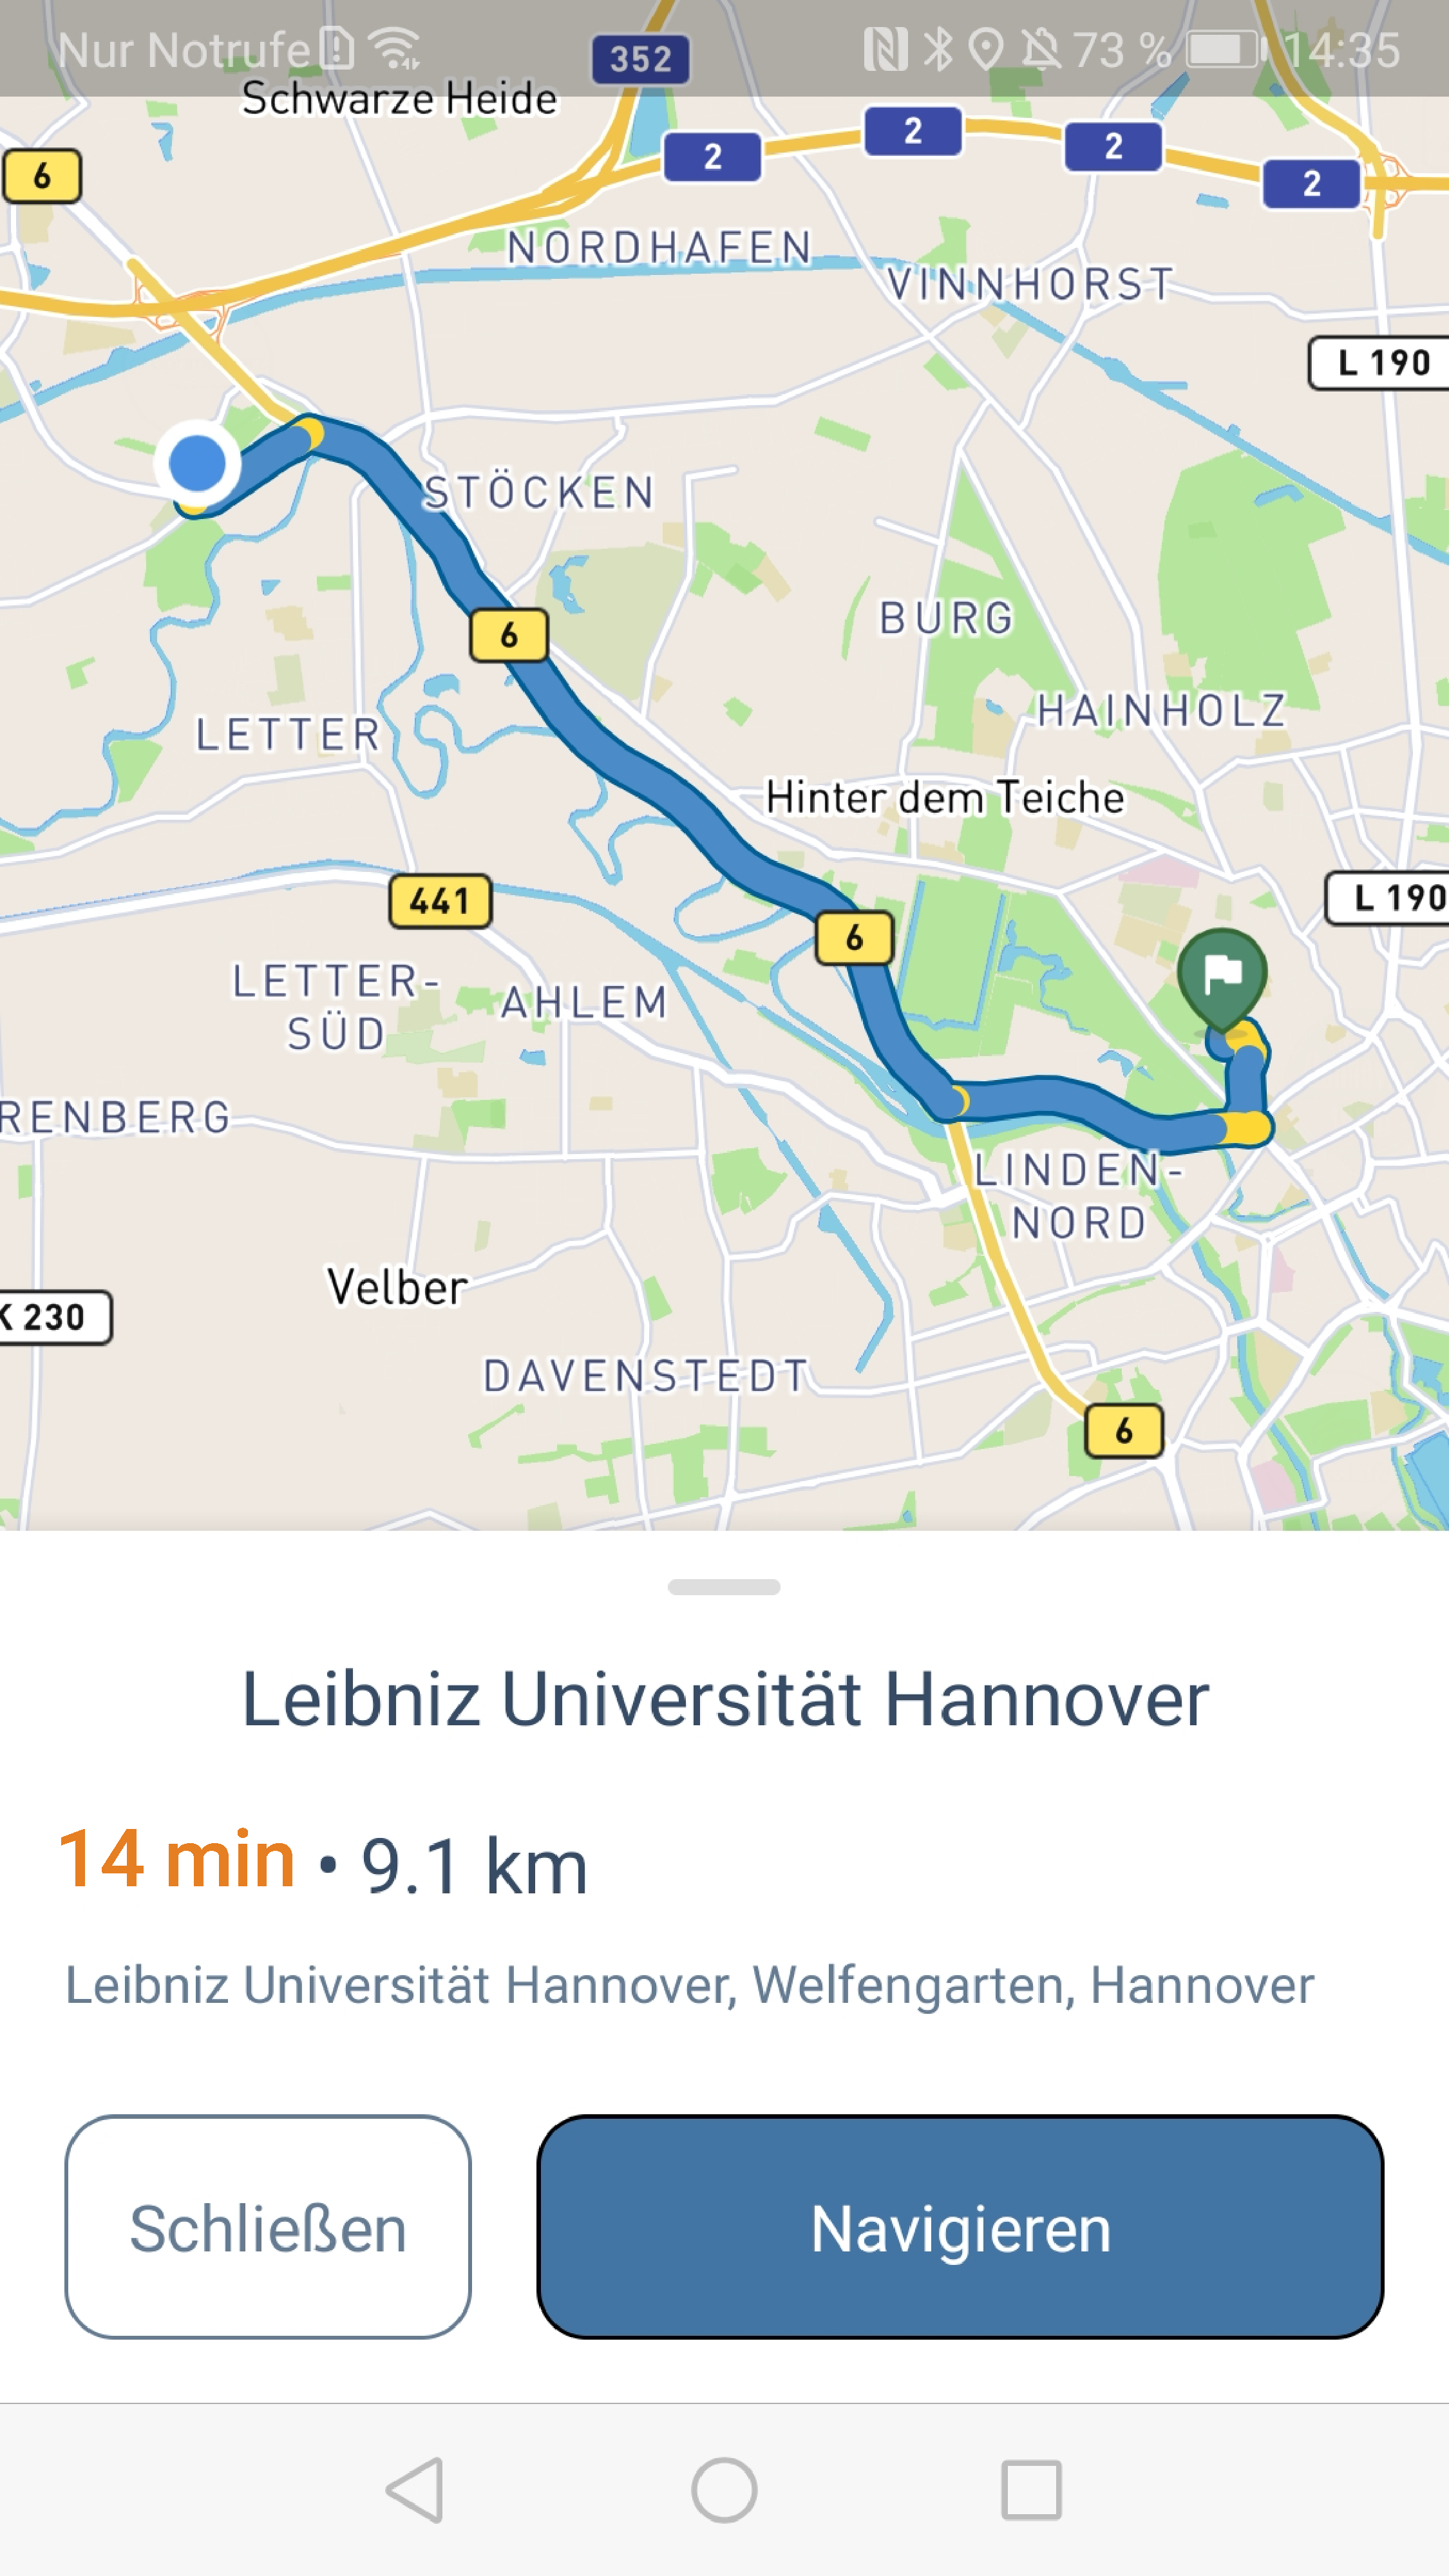
\includegraphics[width=.27\linewidth]{contents/06_model_evaluation/01_integration/res/03_traffic_volume/prototype_11.pdf}
    }
    \hspace{.055\linewidth}
    \subfloat[Alternativer Prototyp zur Positionierung der \textit{Affordance}]
    {
        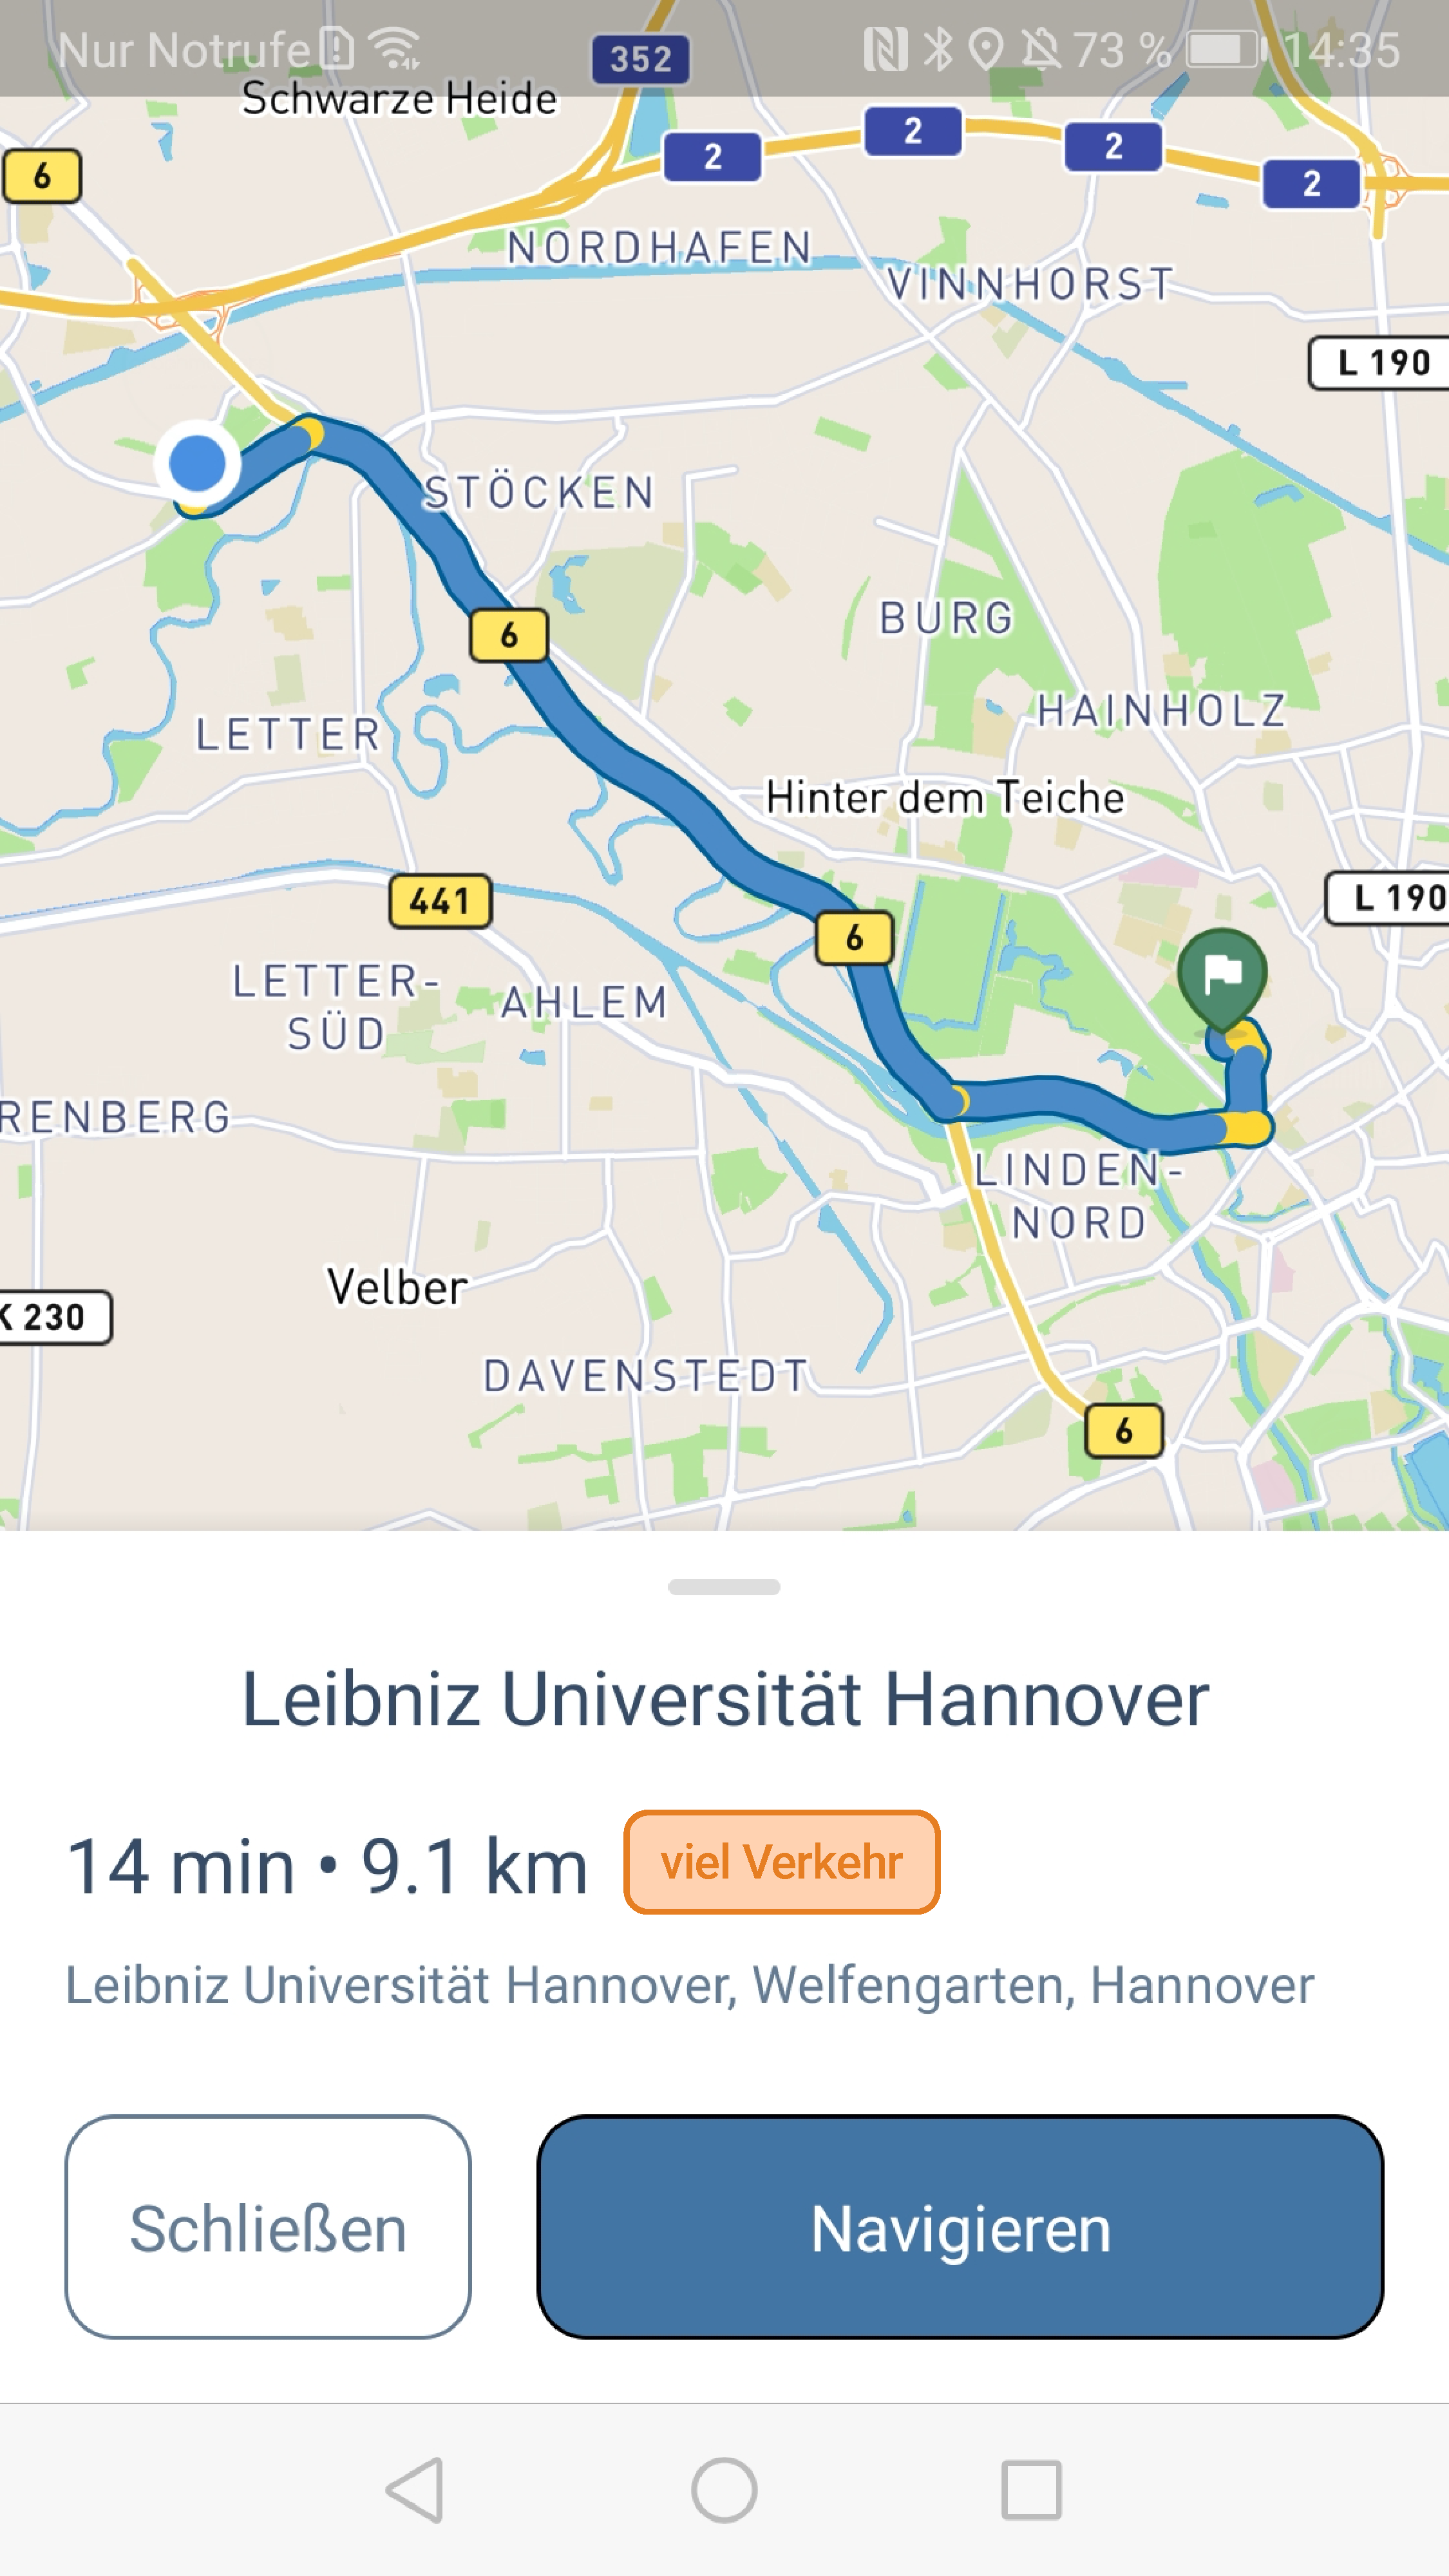
\includegraphics[width=.27\linewidth]{contents/06_model_evaluation/01_integration/res/03_traffic_volume/prototype_12.pdf}
    }
    \hspace{.055\linewidth}
    \subfloat[Finales Design der kurzen Erklärung]
    {
        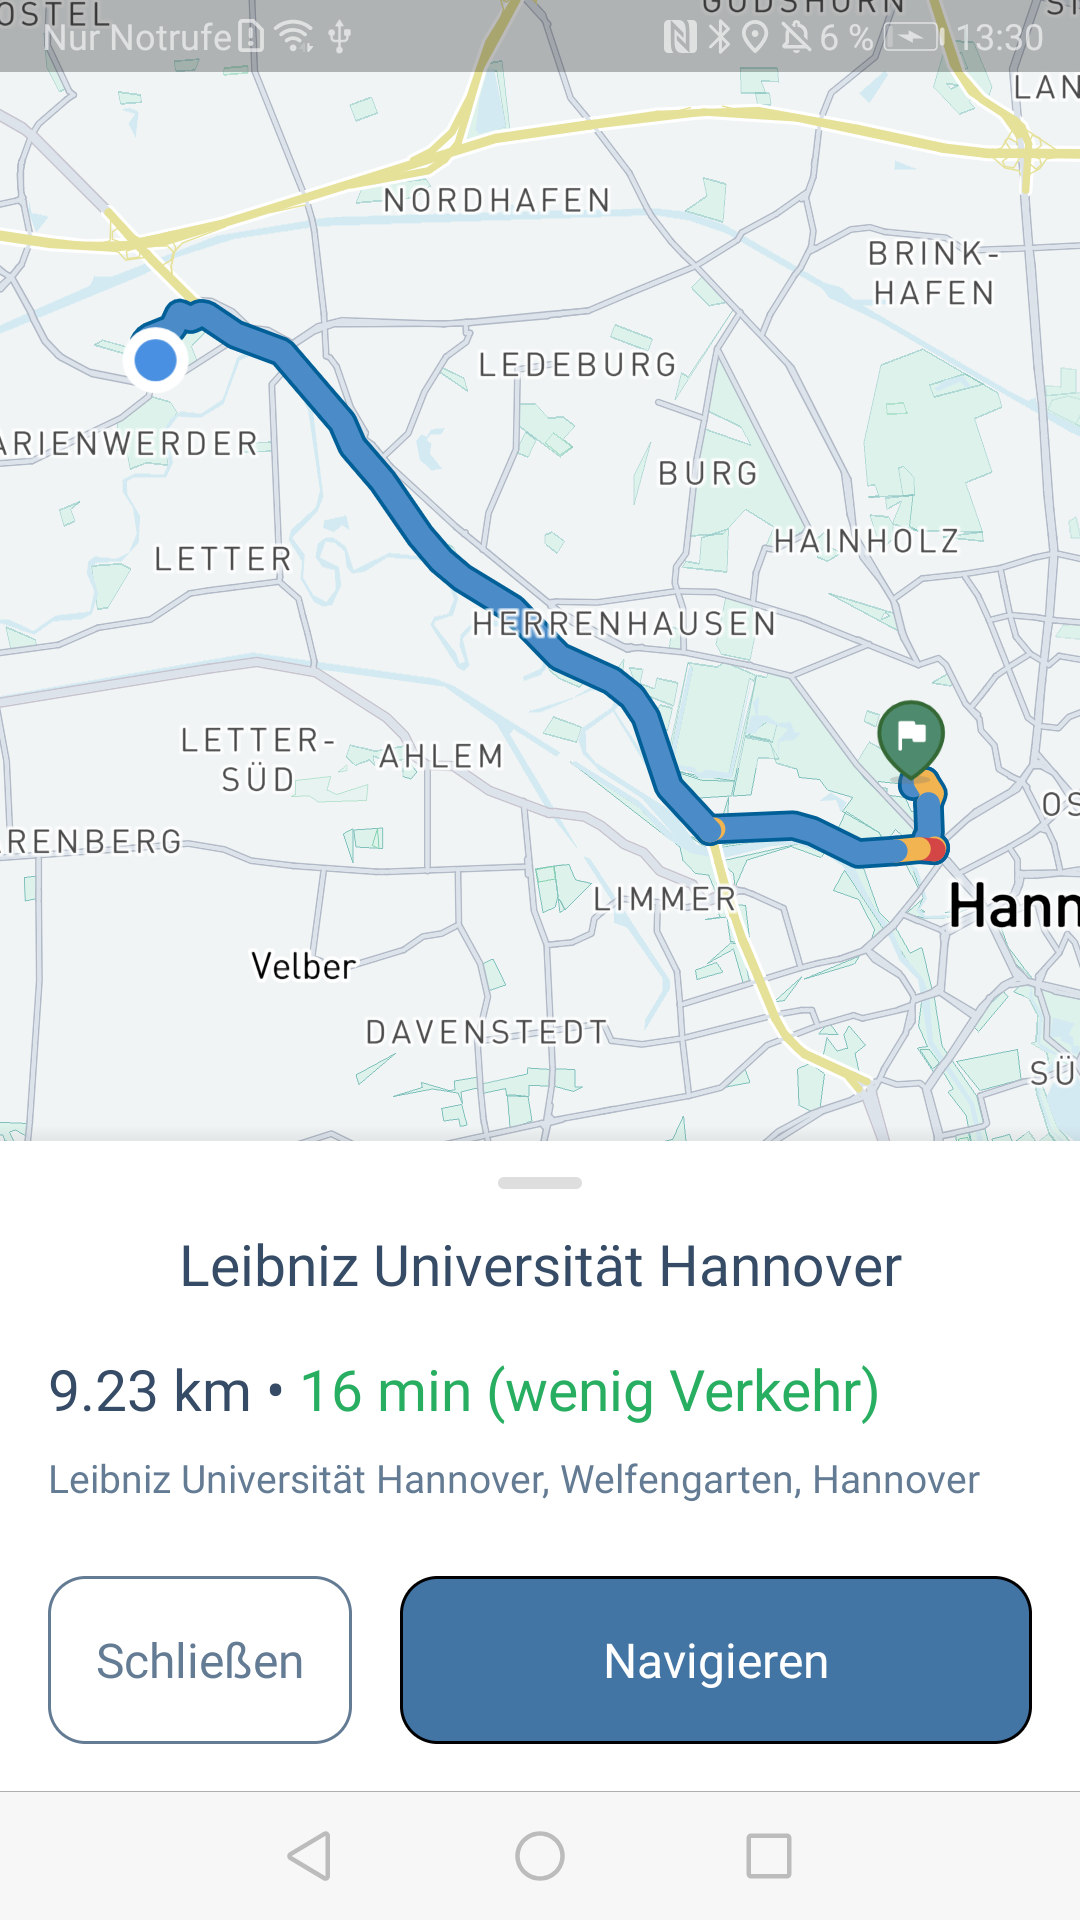
\includegraphics[width=.27\linewidth]{contents/06_model_evaluation/01_integration/res/03_traffic_volume/final_10.png}
    }
    \caption{Prototyp und finale Designs für die Erklärung zum kollaborativem Routing}
    \label{fig:prototype_traffic_volume_route_overview}
\end{figure}

\begin{figure}[htb!]
    \centering
    \subfloat[1. Prototyp zur Positionierung der \textit{Affordance}]
    {
        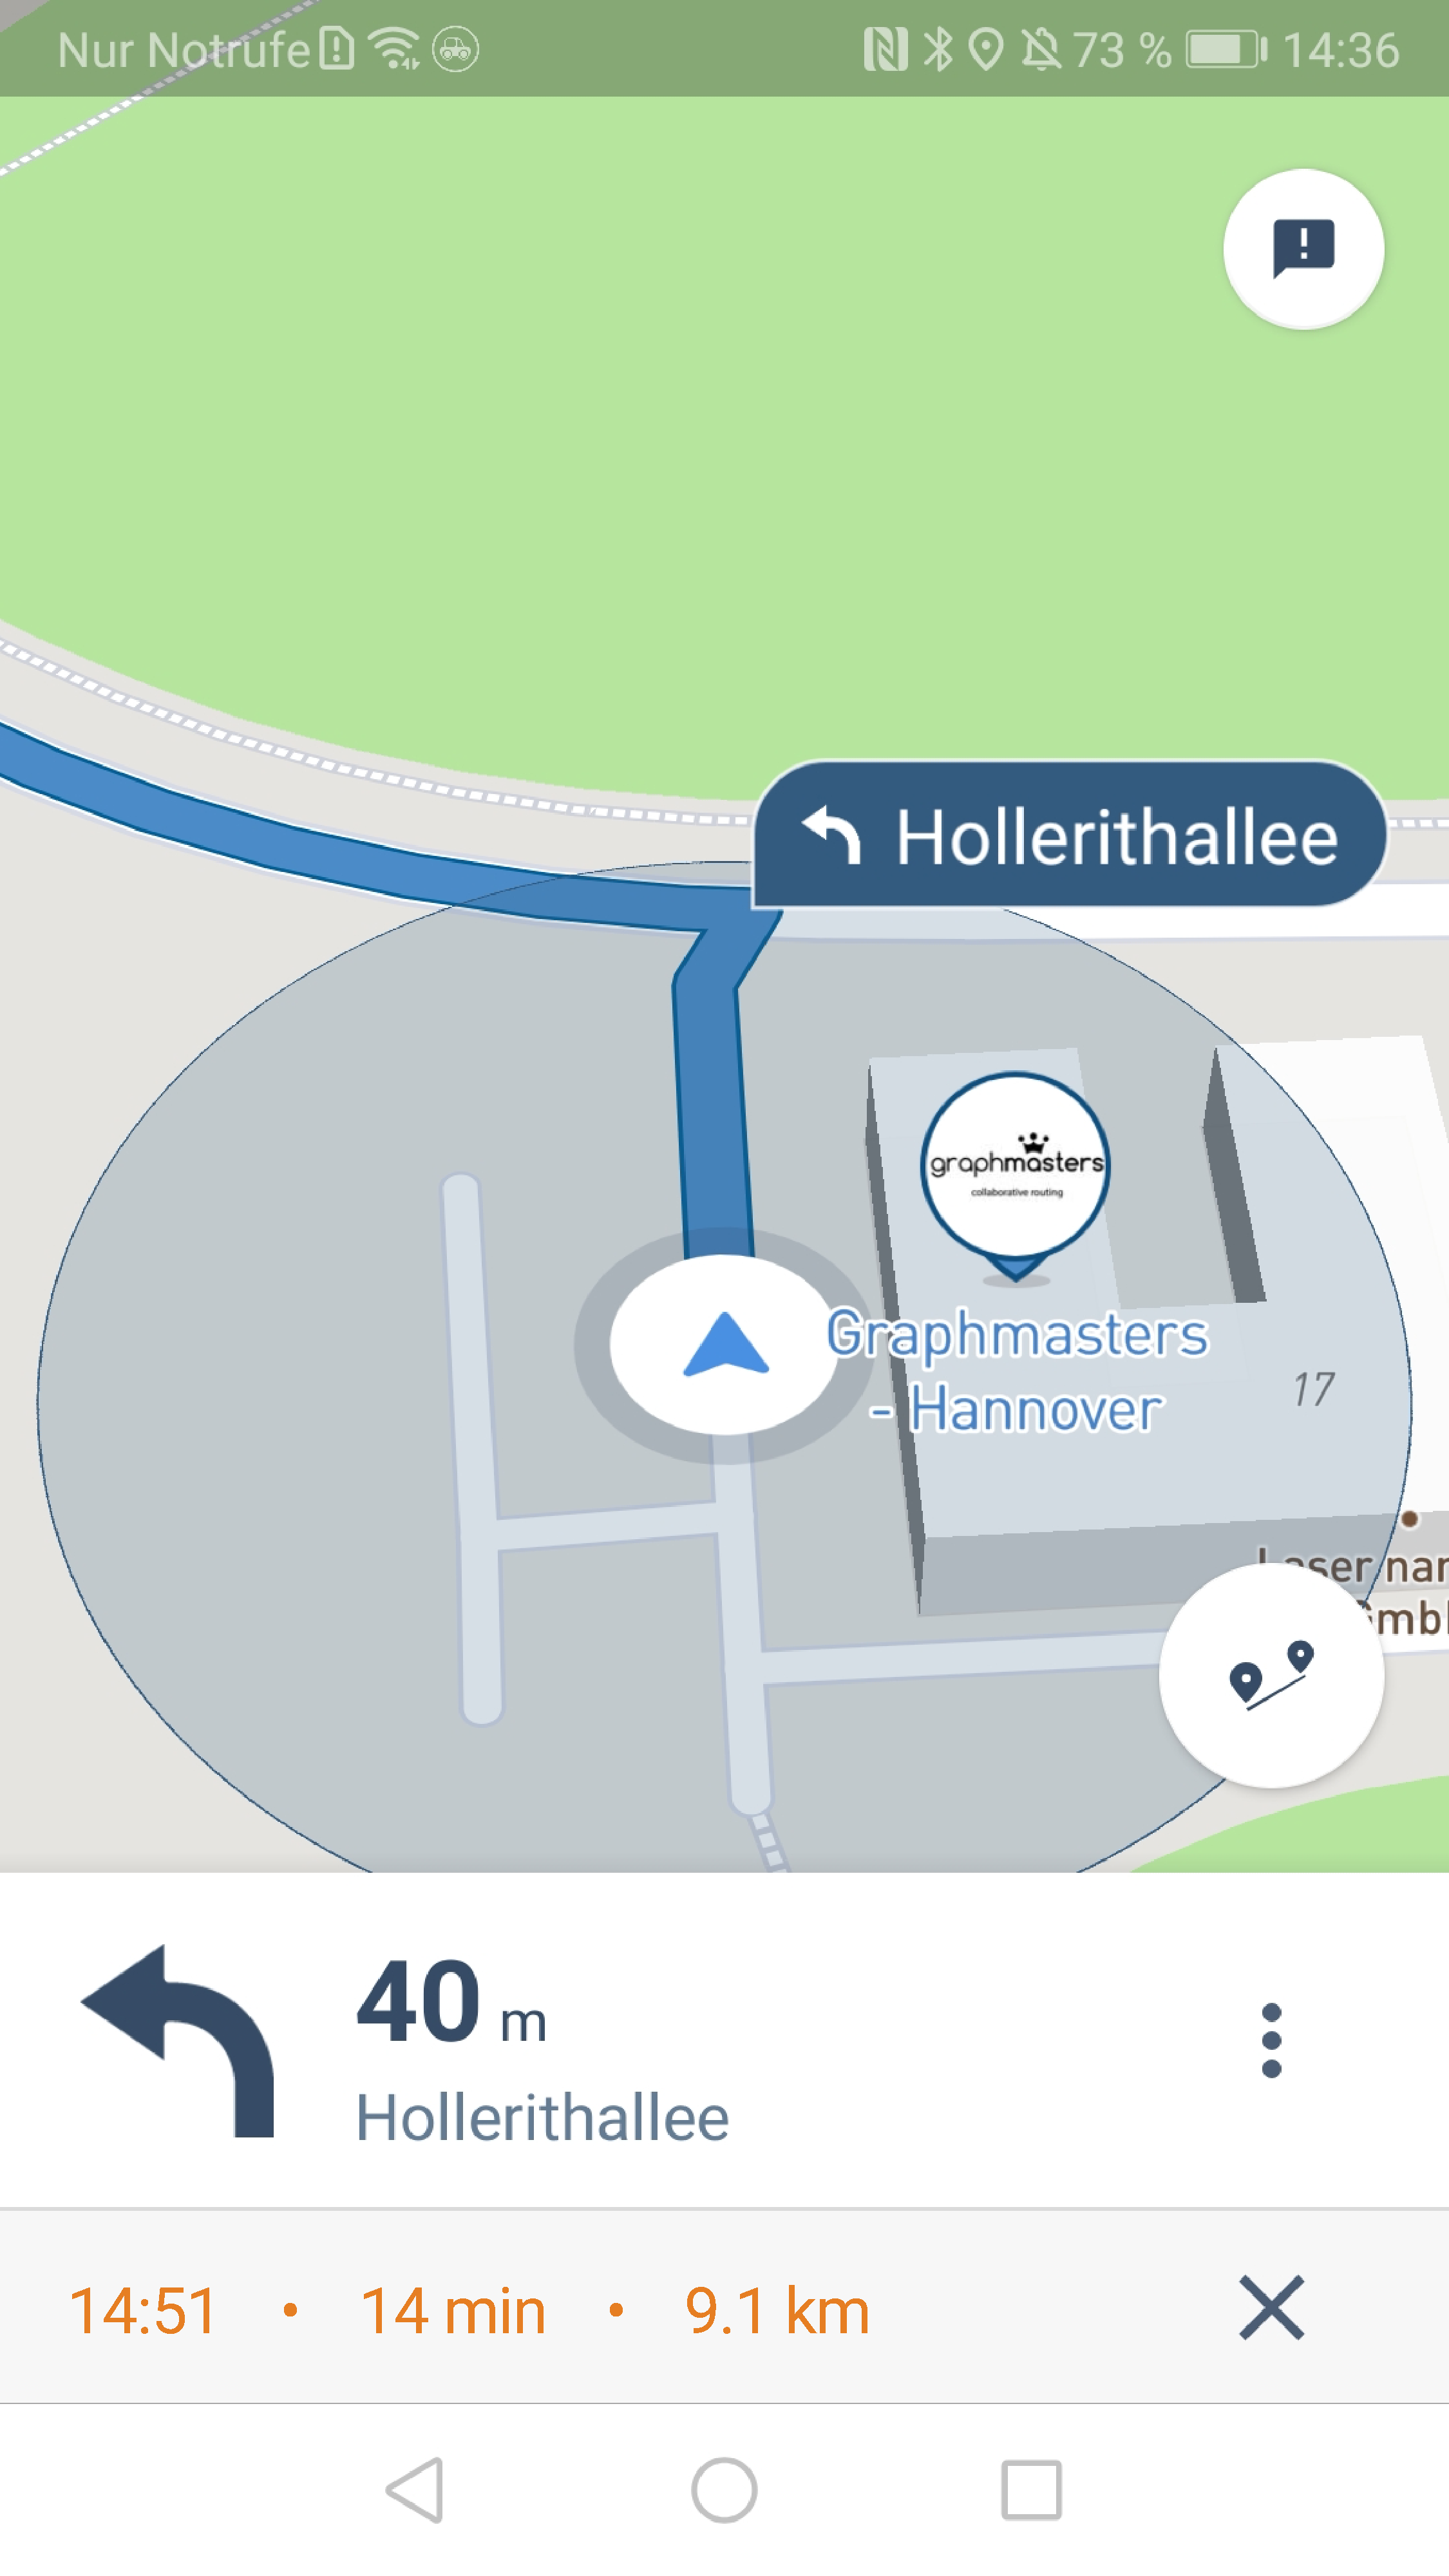
\includegraphics[width=.27\linewidth]{contents/06_model_evaluation/01_integration/res/03_traffic_volume/prototype_21.pdf}
    }
    \hspace{.055\linewidth}
    \subfloat[Alternativer Prototyp zur Positionierung der \textit{Affordance}]
    {
        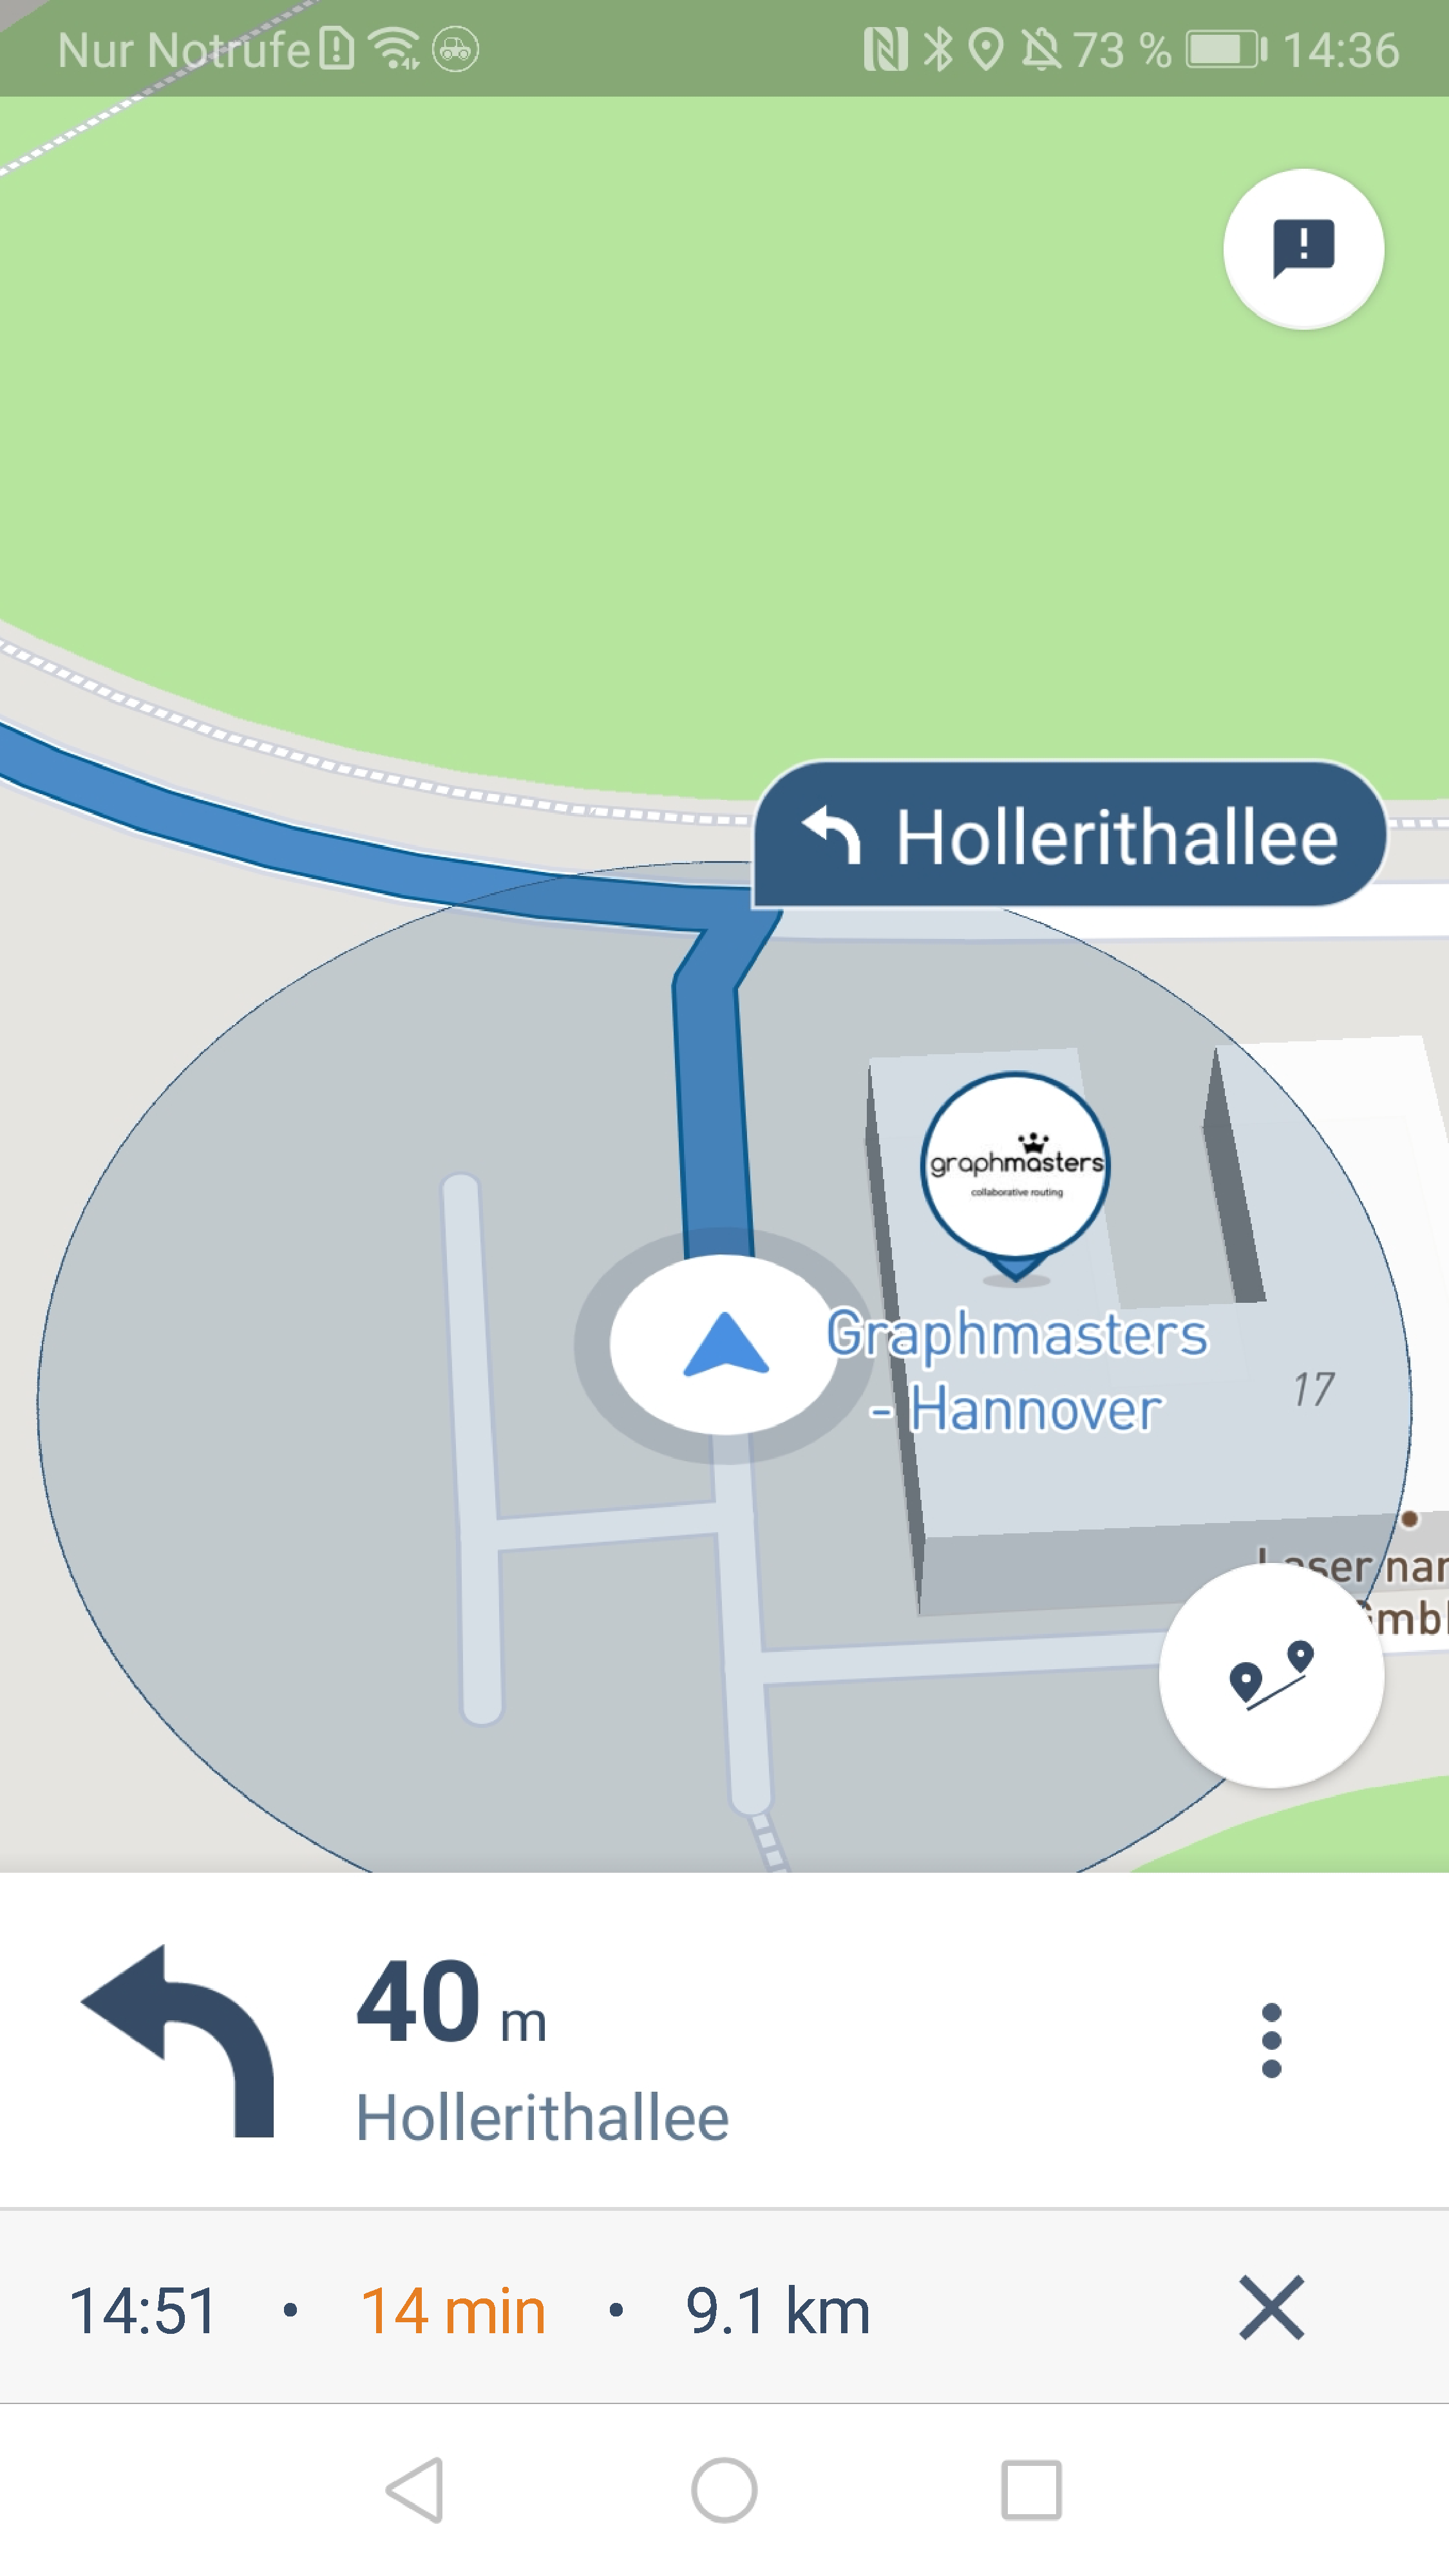
\includegraphics[width=.27\linewidth]{contents/06_model_evaluation/01_integration/res/03_traffic_volume/prototype_22.pdf}
    }
    \hspace{.055\linewidth}
    \subfloat[Finales Design der kurzen Erklärung]
    {
        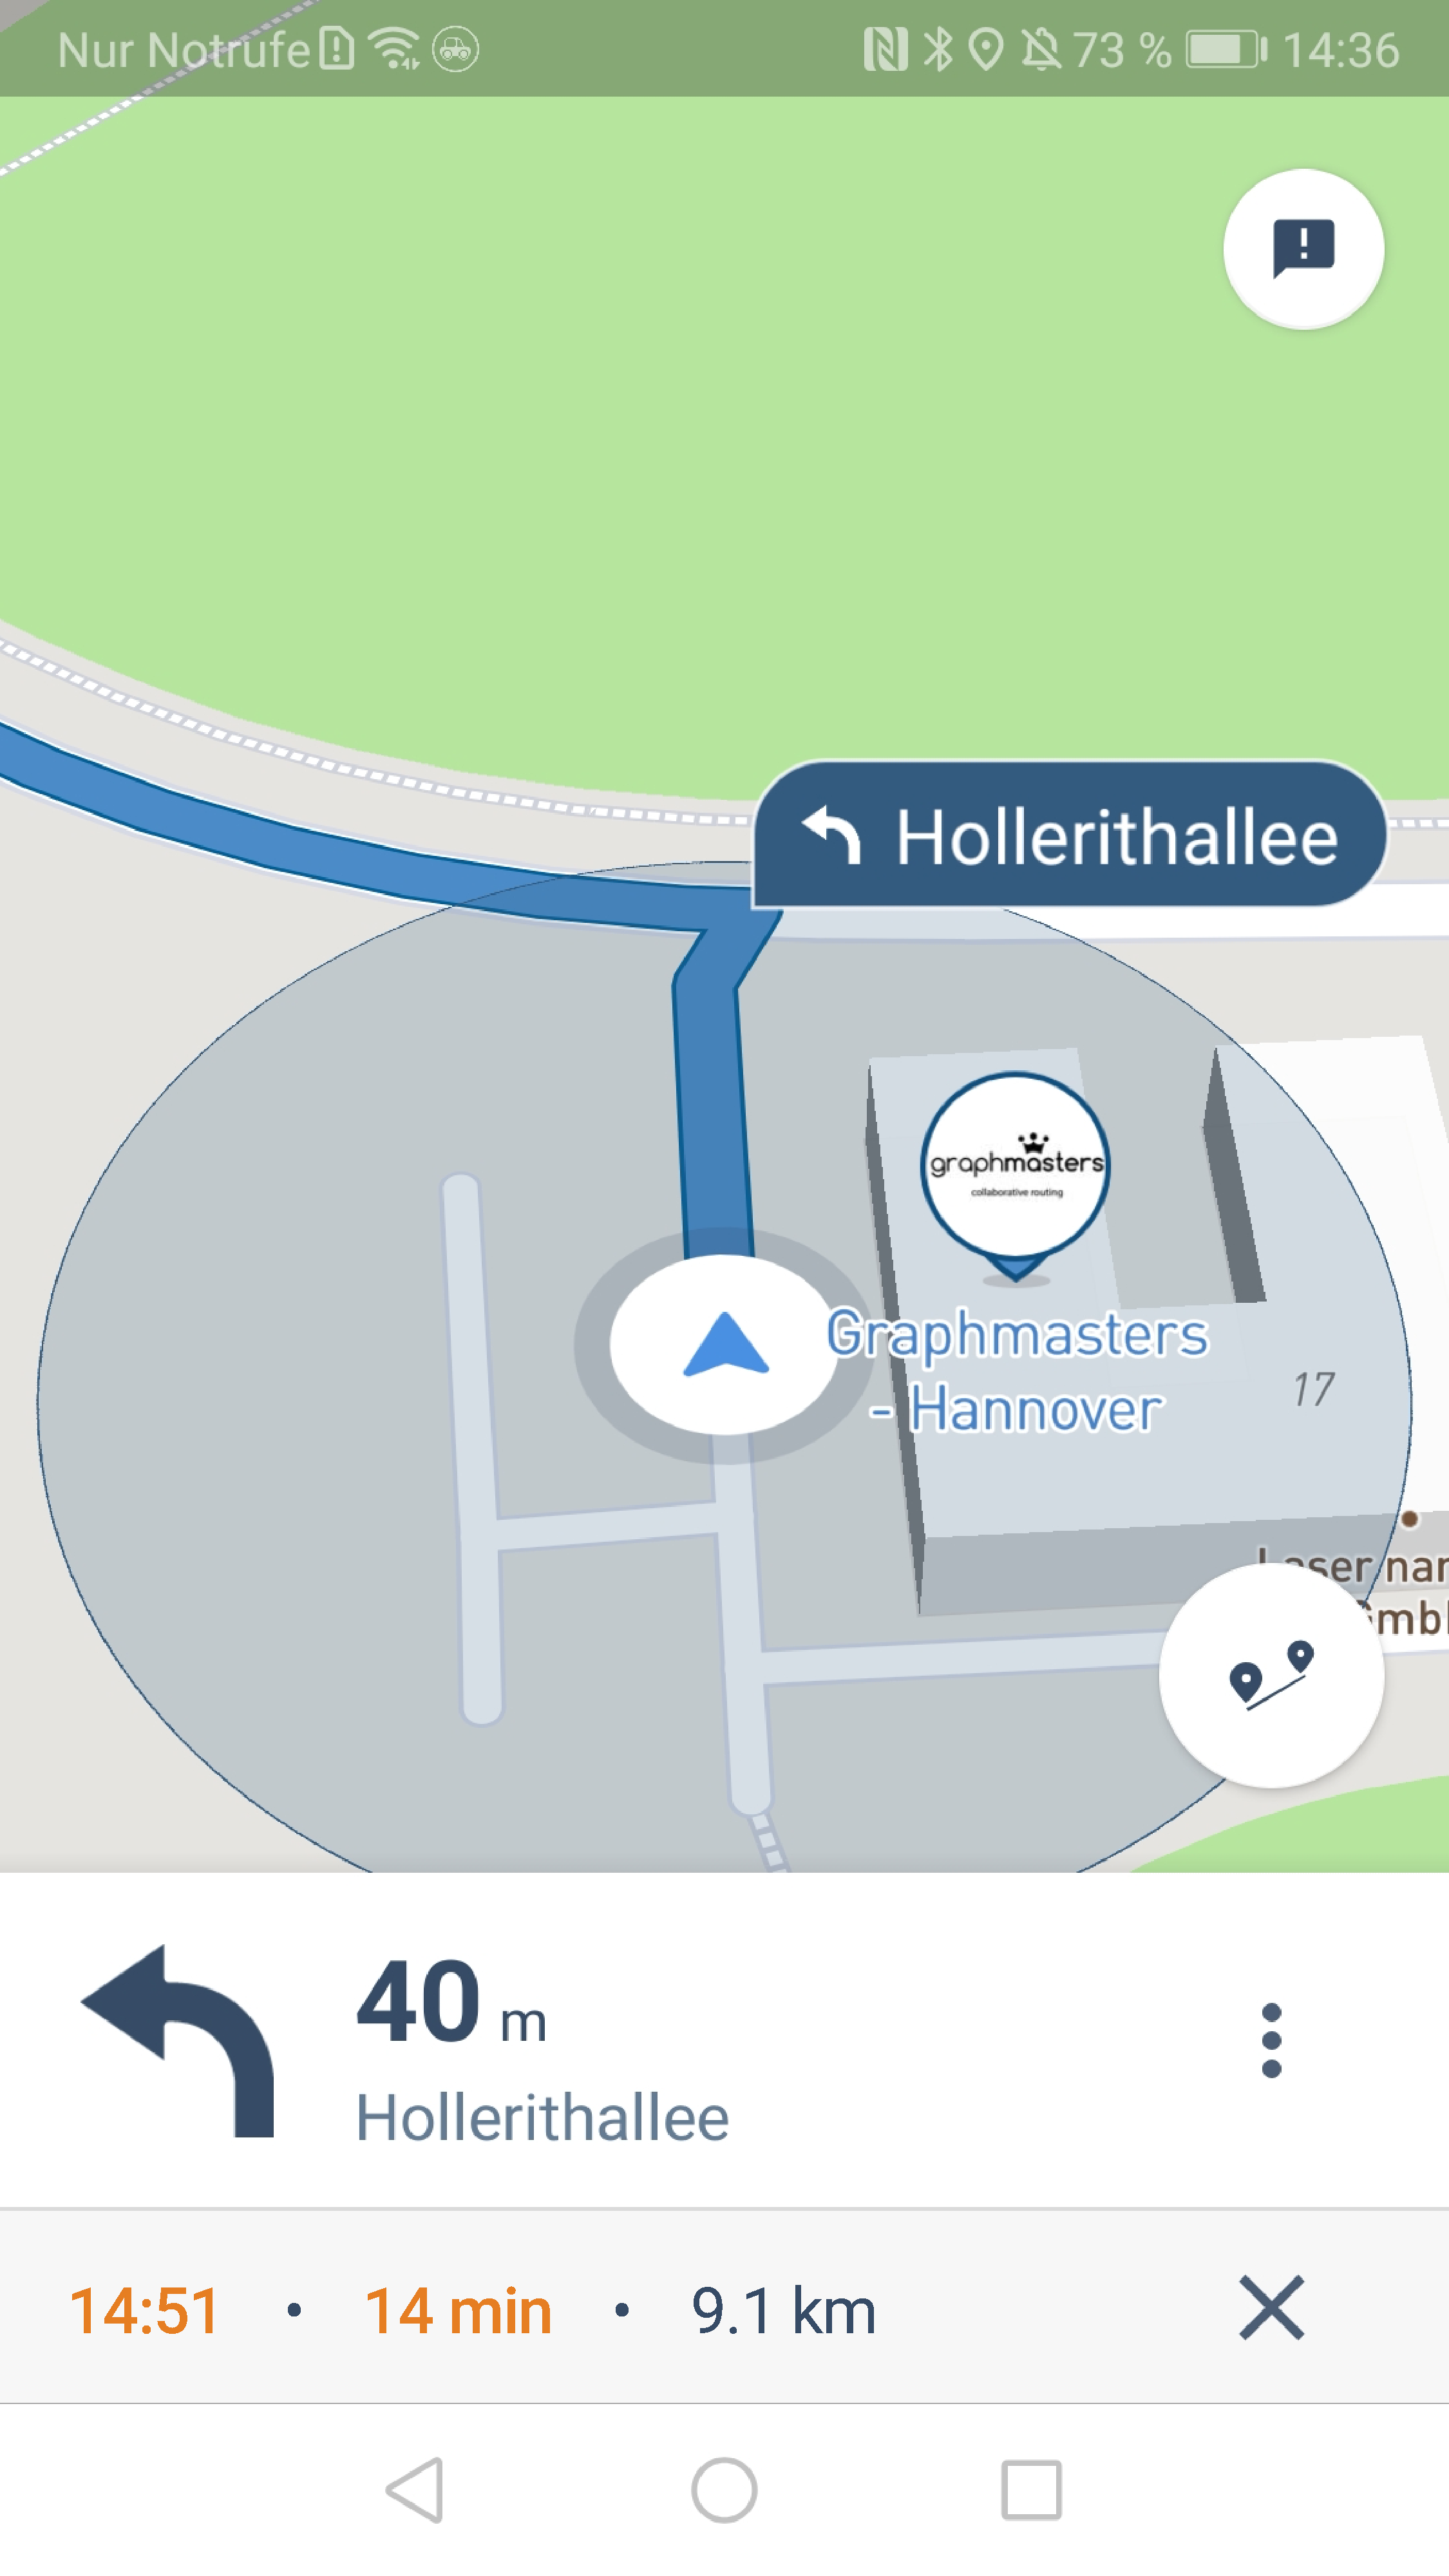
\includegraphics[width=.27\linewidth]{contents/06_model_evaluation/01_integration/res/03_traffic_volume/final_20.pdf}
    }
    \caption{Prototyp und finale Designs für die Erklärung zum kollaborativem Routing}
    \label{fig:prototype_traffic_volume_navigation}
\end{figure}